%% abtex2-modelo-trabalho-academico.tex, v-1.8 laurocesar
%% Copyright 2012-2013 by abnTeX2 group at http://abntex2.googlecode.com/ 
%%
%% This work may be distributed and/or modified under the
%% conditions of the LaTeX Project Public License, either version 1.3
%% of this license or (at your option) any later version.
%% The latest version of this license is in
%%   http://www.latex-project.org/lppl.txt
%% and version 1.3 or later is part of all distributions of LaTeX
%% version 2005/12/01 or later.
%%
%% This work has the LPPL maintenance status `maintained'.
%% 
%% The Current Maintainer of this work is the abnTeX2 team, led
%% by Lauro César Araujo. Further information are available on 
%% http://abntex2.googlecode.com/
%%
%% This work consists of the files abntex2-modelo-trabalho-academico.tex,
%% abntex2-modelo-include-comandos and abntex2-modelo-references.bib
%%

% ------------------------------------------------------------------------
% ------------------------------------------------------------------------
% abnTeX2: Modelo de Trabalho Academico (tese de doutorado, dissertacao de
% mestrado e trabalhos monograficos em geral) em conformidade com 
% ABNT NBR 14724:2011: Informacao e documentacao - Trabalhos academicos -
% Apresentacao
% ------------------------------------------------------------------------
% ------------------------------------------------------------------------

\documentclass[
	% -- opções da classe memoir --
	11pt,				% tamanho da fonte
	openright,			% capítulos começam em pág ímpar (insere página vazia caso preciso)
	oneside,			% twoside para impressão em verso e anverso. Oposto a oneside
	a4paper,			% tamanho do papel. 
	% -- opções da classe abntex2 --
	%chapter=TITLE,		% títulos de capítulos convertidos em letras maiúsculas
	%section=TITLE,		% títulos de seções convertidos em letras maiúsculas
	%subsection=TITLE,	% títulos de subseções convertidos em letras maiúsculas
	%subsubsection=TITLE,% títulos de subsubseções convertidos em letras maiúsculas
	% -- opções do pacote babel --
	english,			% idioma adicional para hifenização
	french,				% idioma adicional para hifenização
	spanish,			% idioma adicional para hifenização
	brazil,				% o último idioma é o principal do documento
	]{abntex2}

\usepackage{abntex2-cefetmg-timoteo}

% ---
% PACOTES
% ---

% ---
% Pacotes fundamentais 
% ---
\usepackage{float}
\usepackage{cmap}				% Mapear caracteres especiais no PDF
\usepackage{lmodern}			% Usa a fonte Latin Modern			
\usepackage[T1]{fontenc}		% Selecao de codigos de fonte.
\usepackage[utf8]{inputenc}		% Codificacao do documento (conversão automática dos acentos)
\usepackage{lastpage}			% Usado pela Ficha catalográfica
\usepackage{indentfirst}		% Indenta o primeiro parágrafo de cada seção.
\usepackage{color}				% Controle das cores
\usepackage{graphicx}			% Inclusão de gráficos
\PassOptionsToPackage{normalem}{ulem} % Para não usar sublinhado em referências bibliográficas
\usepackage{ulem}
\usepackage{multicol}

% ---

%Trocar fonte para Arial ou Helvetica
%\usepackage{uarial}
\usepackage{helvet}
\renewcommand{\familydefault}{\sfdefault}

		
% ---
% Pacotes adicionais, usados apenas no âmbito do Modelo Canônico do abnteX2
% ---
%\usepackage{lipsum}				% para geração de dummy text
% ---

% ---
% Pacotes de citações
% ---
\usepackage[brazilian,hyperpageref]{backref}	 % Paginas com as citações na bibl
\usepackage[alf,abnt-thesis-year=both,]{abntex2cite}	% Citações padrão ABNT


%Outros pacotes

\usepackage{longtable}


%\setlrmarginsandblock{3cm}{2cm}{*}
%\setulmarginsandblock{3cm}{2cm}{*}
%\checkandfixthelayout


% --- 
% CONFIGURAÇÕES DE PACOTES
% --- 

% ---
% Configurações do pacote backref
% Usado sem a opção hyperpageref de backref
\renewcommand{\backrefpagesname}{Citado na(s) página(s):~}
% Texto padrão antes do número das páginas
\renewcommand{\backref}{}
% Define os textos da citação
\renewcommand*{\backrefalt}[4]{
	\ifcase #1 %
		Nenhuma citação no texto.%
	\or
		Citado na página #2.%
	\else
		%Citado #1 vezes nas páginas #2.%
		Citado nas páginas #2.%
	\fi}%
% ---


% ---
% Informações de dados para CAPA e FOLHA DE ROSTO
% ---
\titulo{PRNG \\(PSEUDORANDOM NUMBER GENERATORS)}
\autor{João Pedro Pereira de Assis Castro Santos \\Juliana Silva Cruz Sartori}
\local{Timóteo}
\data{2022}
\orientador{Gustavo Henrique Borges Martins}

\instituicao{%
  Centro Federal de Educação Tecnológica de Minas Gerais
  \par
  Campus Timóteo
  \par
  Graduação em Engenharia de Computação
}



% ---

% ---
% Configurações de aparência do PDF final

% informações do PDF
\makeatletter
\hypersetup{
     	%pagebackref=true,
		pdftitle={\@title}, 
		pdfauthor={\@author},
    	pdfsubject={\imprimirpreambulo},
	    pdfcreator={LaTeX with abnTeX2},
		pdfkeywords={abnt}{latex}{abntex}{abntex2}{trabalho acadêmico}, 
		colorlinks=true,       		% false: boxed links; true: colored links
    	linkcolor=black,          	% color of internal links
    	citecolor=black,        		% color of links to bibliography
    	filecolor=black,      		% color of file links
		urlcolor=black,
		bookmarksdepth=4
}
\makeatother
% --- 

% --- 
% Espaçamentos entre linhas e parágrafos 
% --- 

% O tamanho do parágrafo é dado por:
\setlength{\parindent}{1.3cm}

% Controle do espaçamento entre um parágrafo e outro:
\setlength{\parskip}{0.1cm}  % tente também \onelineskip

% ---
% compila o indice
% ---
\makeindex
% ---

% ----
% Início do documento
% ----
\begin{document}

% Retira espaço extra obsoleto entre as frases.
\frenchspacing 

% ----------------------------------------------------------
% ELEMENTOS PRÉ-TEXTUAIS
% ----------------------------------------------------------
 \pretextual

% ---
% Capa
% ---
\imprimircapa
% ---






% ----------------------------------------------------------
% ELEMENTOS TEXTUAIS
% ----------------------------------------------------------
\textual

% ----------------------------------------------------------
% Introdução
% ----------------------------------------------------------
\chapter[Introdução]{Introdução}
A geração de números aleatórios tem muitos usos (em sua maioria em estatística, para amostragem aleatória e simulação). Antes da computação moderna, pesquisadores que precisavam de números aleatórios os gerava através de vários meios (dado, cartas, roleta, etc.), ou utilizavam as tabelas de números aleatórios existentes.
A primeira tentativa de prover para os pesquisadores um suprimento pronto de dígitos aleatórios foi feita em 1927, quando a Cambridge University Press publicou uma tabela de 41.600 dígitos desenvolvida por Leonard H.C. Tippet. Em 1947, a RAND Corporation gerou números por meio de uma simulação eletrônica de uma roleta; os resultados foram eventualmente publicados em 1955 como A Million Random Digits with 100,000 Normal Deviates (Um milhão de dígitos aleatórios com 100.000 desvios normais).\cite{Sit}

John von Neumann foi um pioneiro dos geradores de números aleatórios baseados em computadores. Um contribuidor notável no campo da geração de números pseudoa leatórios para uso prático, é um matemático paquistanês Dr. Arif Zaman. Em 1951, Derrick Henry Lehmer inventou o gerador linear congruente, utilizado na maioria dos geradores de números pseudoa leatórios atuais. Com a disseminação do uso dos computadores, geradores de números pseudoa leatórios substituíram as tabelas numéricas, e "verdadeiros" geradores aleatórios (hardwares geradores de números pseudoa leatórios) são utilizados apenas em alguns casos.\cite{Sit}

Uma variável pseudo aleatória é uma variável que é criada por um procedimento determinístico (frequentemente um programa de computador ou uma subrotina) que (geralmente) recebe bits aleatórios como entrada. A cadeia pseudoaleatória irá, tipicamente, ser maior do que a cadeia aleatória original, porém menos aleatória (menor entropia, no sentido aplicado na teoria da informação). Isto pode ser útil para algoritmos aleatórios.
Geradores de números pseudoa leatórios são amplamente utilizados em aplicações como modelagem computacional (e.g., Cadeias de Markov), estatística, design experimental, etc. Alguns deles são suficientemente aleatórios para serem úteis nestas aplicações; muitos não são, e uma sofisticação considerável é necessária para determinar corretamente a diferença para qualquer propósito em particular. O uso não-precavido de geradores de números pseudoa leatórios prontamente disponíveis tem causado danos consideráveis, e por muito tempo sustentados, no valor de um grande número de projetos de pesquisas por muitos anos.\cite{Sit}

%%%%%%%%%%%%%%%%%%%%%%%%%%%%%%%%%%%%%%%%%%%%%%%%%%%%%%%%%%%%%%%%%%%%%%%%%%%%%%%%%%%%%%%%%%%%%%%
% ----------------------------------------------------------
% Desenvolvimento
% ----------------------------------------------------------
\chapter[Desenvolvimento]{Desenvolvimento}
\label{desenvolvimento}
O código XorShift é baseado em mudanças de posição nos bits ou bit shifts. O algoritmo implementado usa a operação de shift para fazer três movimentações nos bits do valor binário da semente, em seguida soma o resultado de tais shifts a um incremento, também advindo da semente somada ao valor Long 123456789L, e faz sua divisão pelo valor máx(número máximo de bits do valor “randomizado”) pela operação \%(módulo), a fim de entregar o resto da divisão como valor final. Caso o valor seja negativo, ele é multiplicado por -1 antes de ser retornado.
\\
Abaixo segue o código implementado:
\begin{figure}[H]
            \centering
                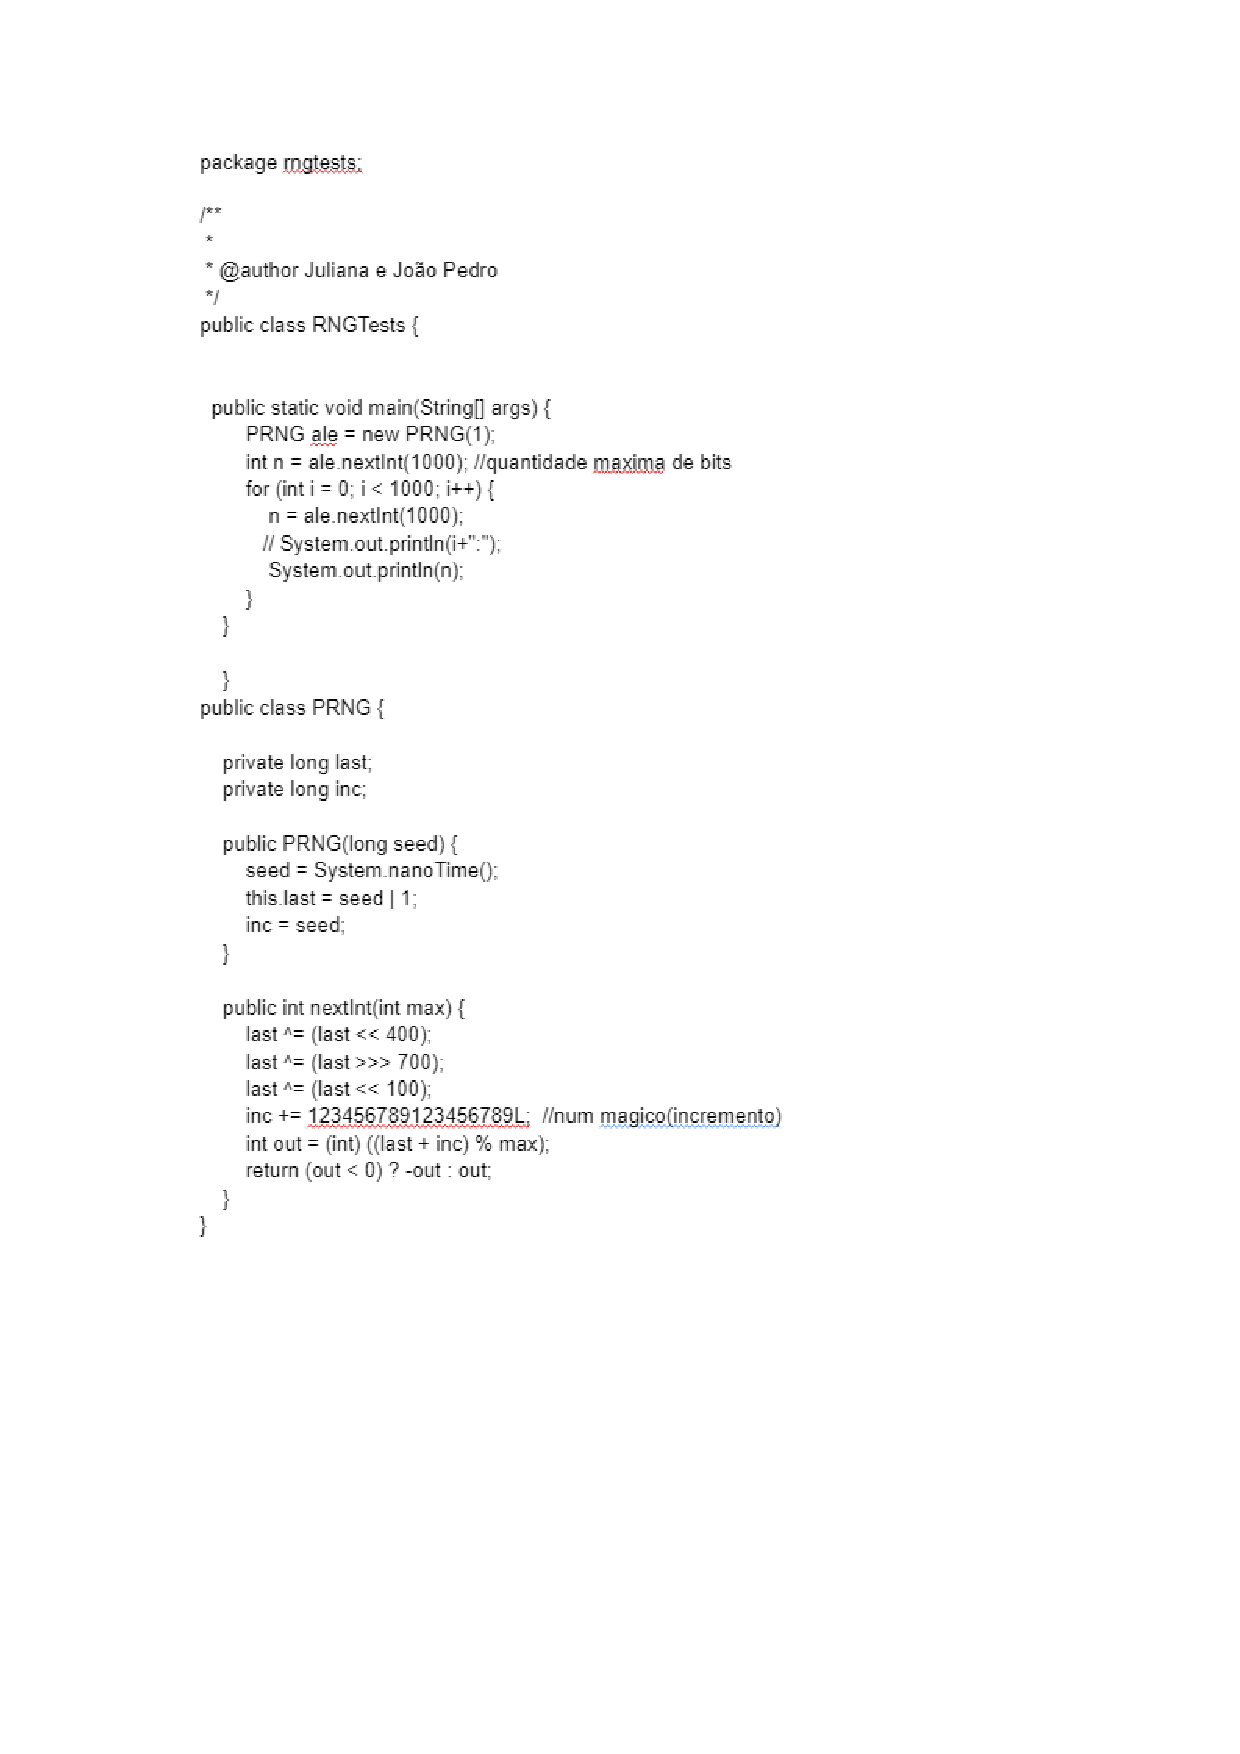
\includegraphics[width=0.72\textwidth]{codigorandom1.pdf}
                \caption{XorShift produzido}
                \label{fig:Desempenho}
        \end{figure} 
A fim de responder a pergunta “O que difere o algoritmo em estudo do Java.util.Random”, devemos compará-los.

O algoritmo da biblioteca java combina o código de gerador do tipo Xorshift com um gerador congruencial a fim de diversificar os resultados o máximo possível:

\begin{figure}[H]
            \centering
                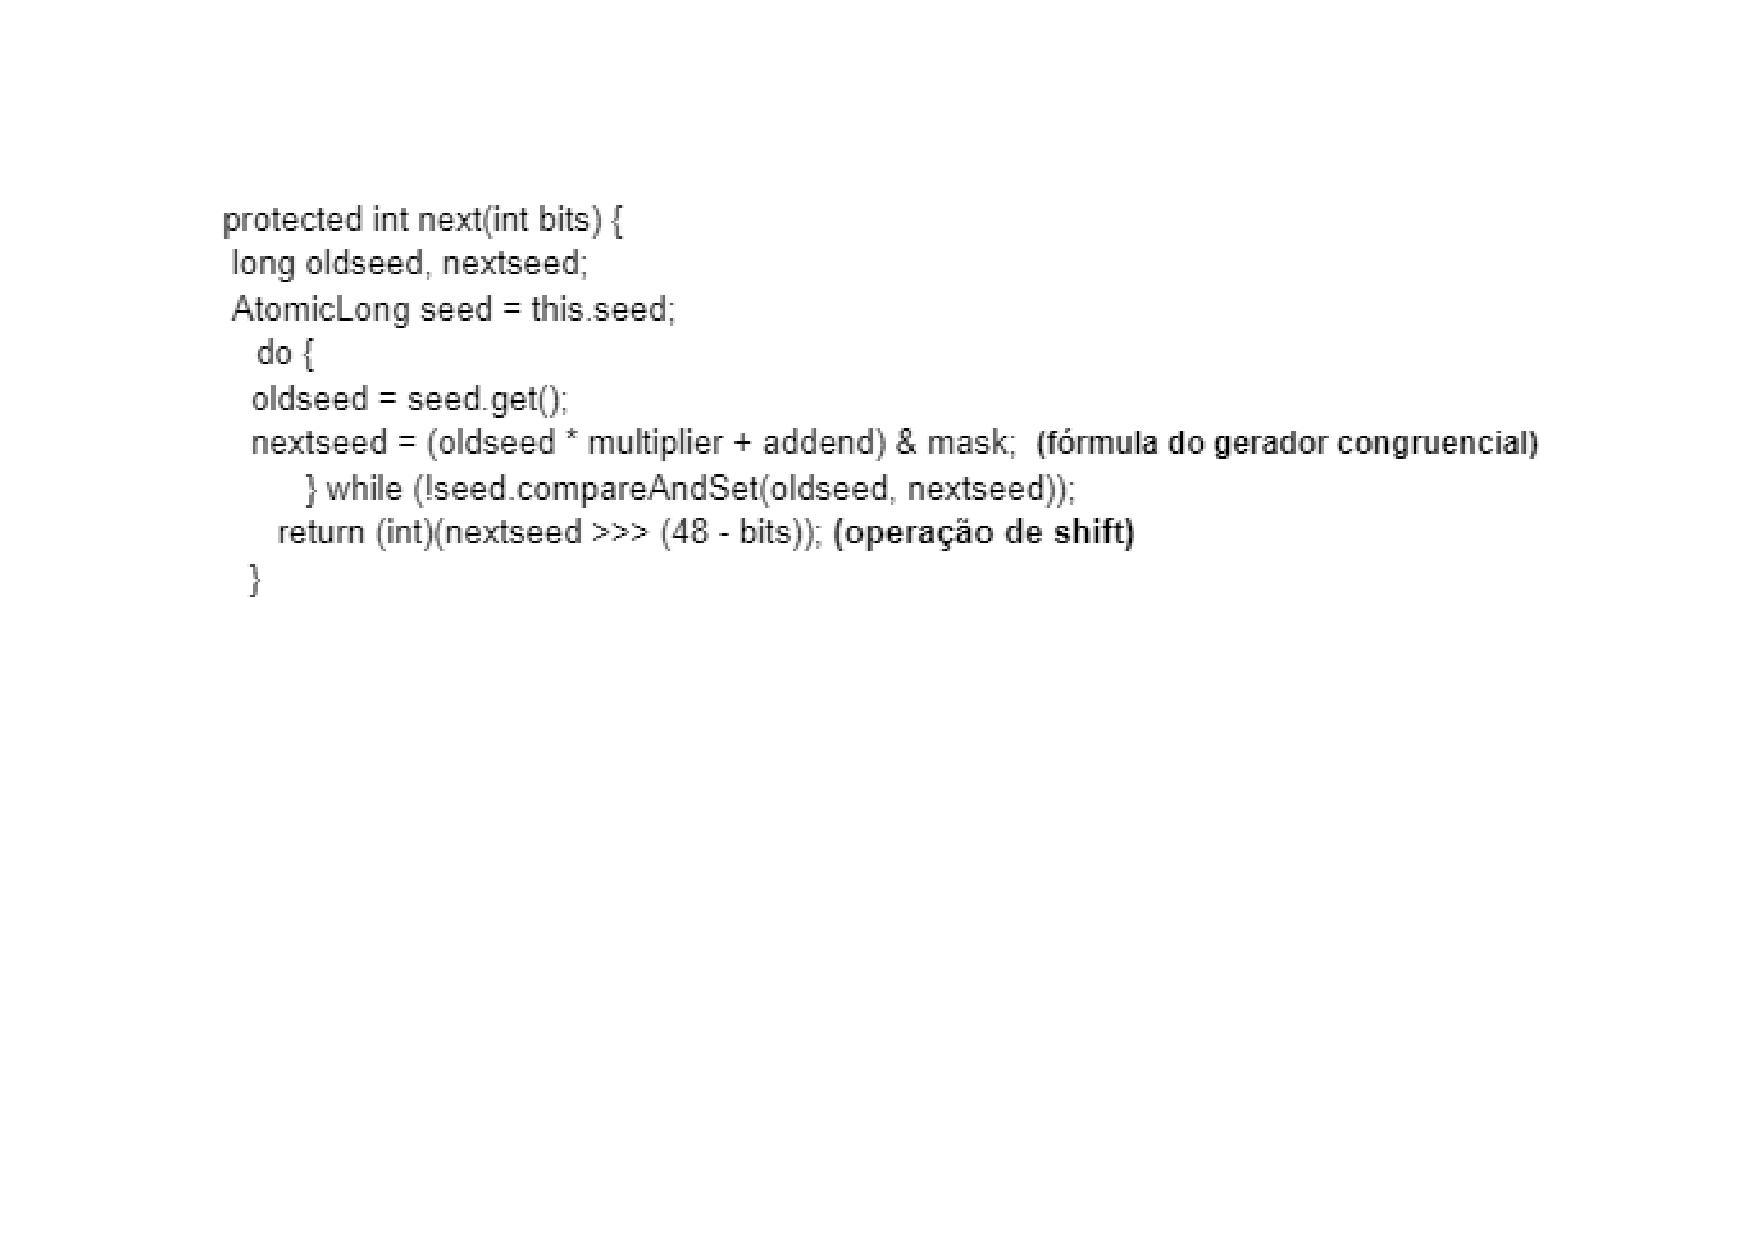
\includegraphics[width=0.74\textwidth]{codigorandomjava.pdf}
                 \caption{Java.util.Random(Gerador pseudo aleatório)}
                \label{fig:Desempenho}
        \end{figure} 

Ambos utilizam como seed(semente) o valor obtido usando System.nanoTime. O código implementado tem ordem de complexidade de tempo O(n) já que executa as chamadas de uma função  O(1)  n vezes dentro de um “for”. O código util.Random do java tem complexidade de O(1) por fazer chamadas do método nextInt que também é O(1) -ele só é executado uma vez, a não ser que o valor resultante seja igual à semente que o originou-, se for utilizado também n  vezes em um laço de repetição, terá também complexidade O(n), logo suas complexidades de tempo são iguais.
Após testes imprimindo vários valores com o loop até o algoritmo começar a repetir uma mesma sequência “randomizada”, encontramos o período de 144 com a execução do código xorshift, o que é igual a $2^{7}$+16, enquanto segundo a wikipédia \cite{SitWik} o período do algoritmo util.Random é de cerca de $2^{32}$ o que indica que o código util.Random pode retornar valores mais variados e menos previsíveis, devido ao período  maior de variabilidade antes de sofrer repetições garantidas.\cite{SitWik}\\       
\\
\\
\\
\\
\\
\\
\\
\\
\\
TABELA: XORSHIFT
\begin{figure}[H]
            \centering
                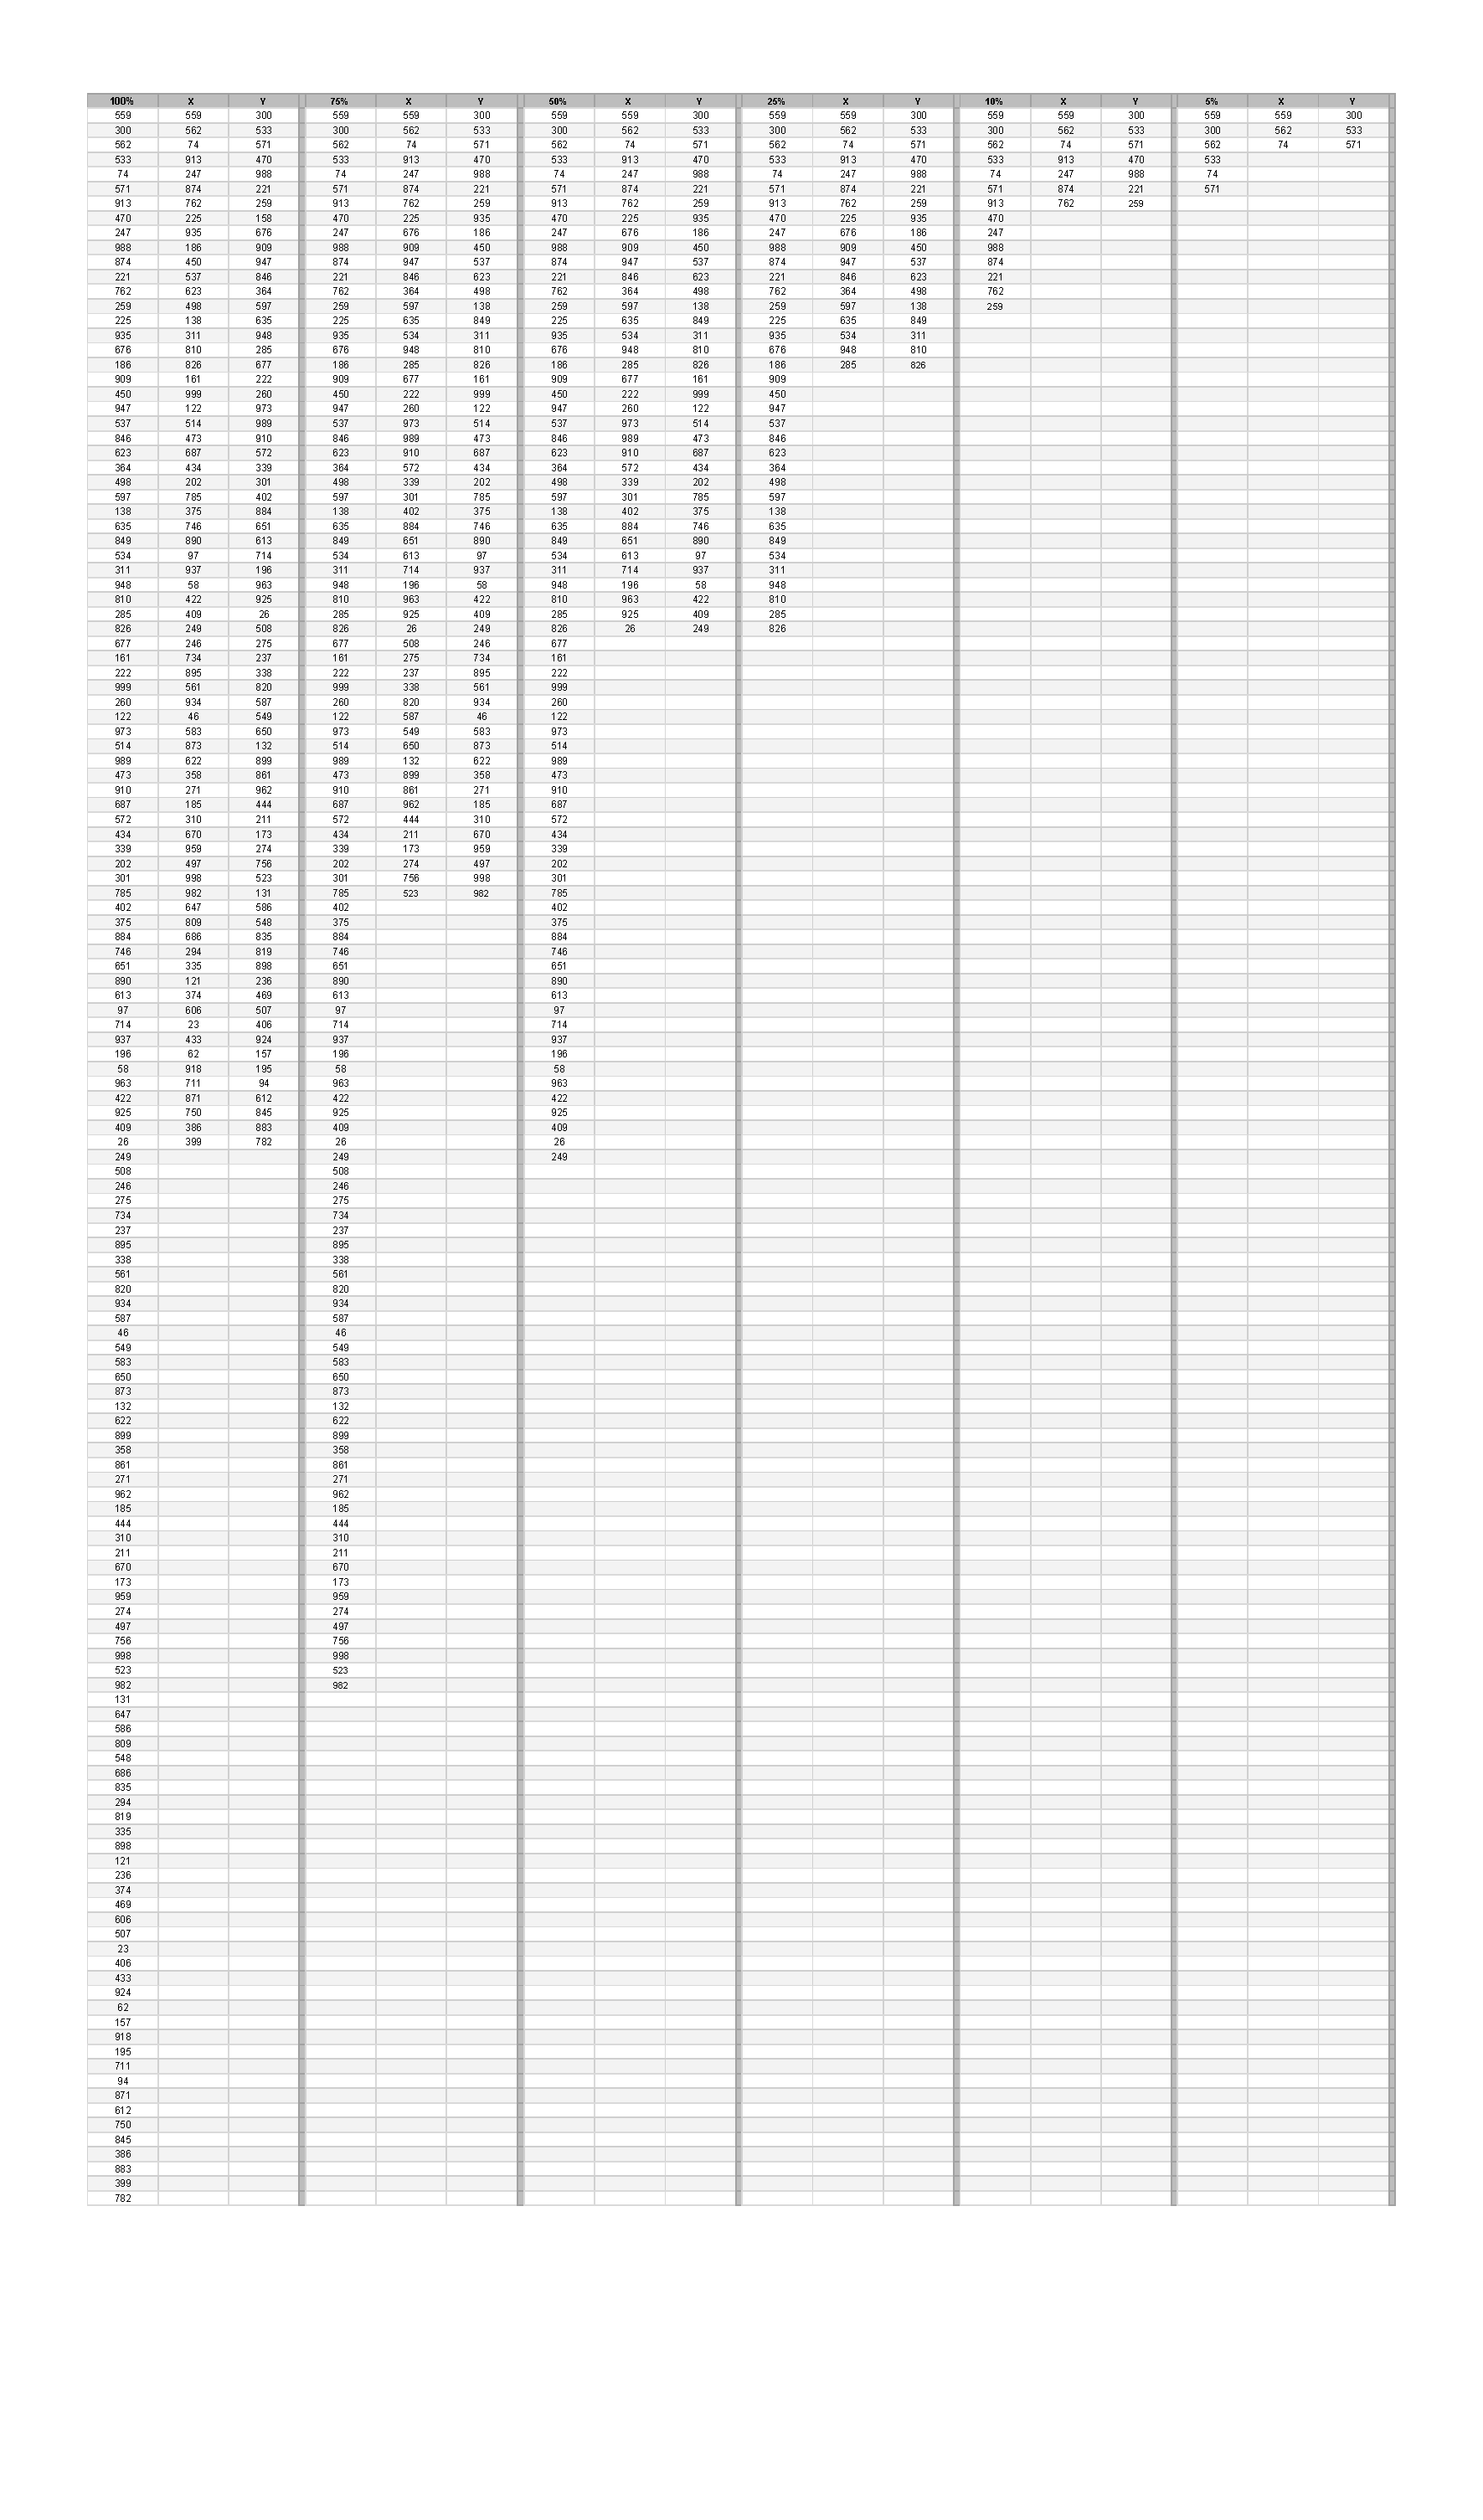
\includegraphics[width=0.84\textwidth]{tabelaExecXorShift.pdf}
                \caption{Valores obtidos em um período}
                \label{fig:Desempenho}
        \end{figure}

TABELA: JAVA.UTIL.RANDOM
\begin{figure}[H]
            \centering
                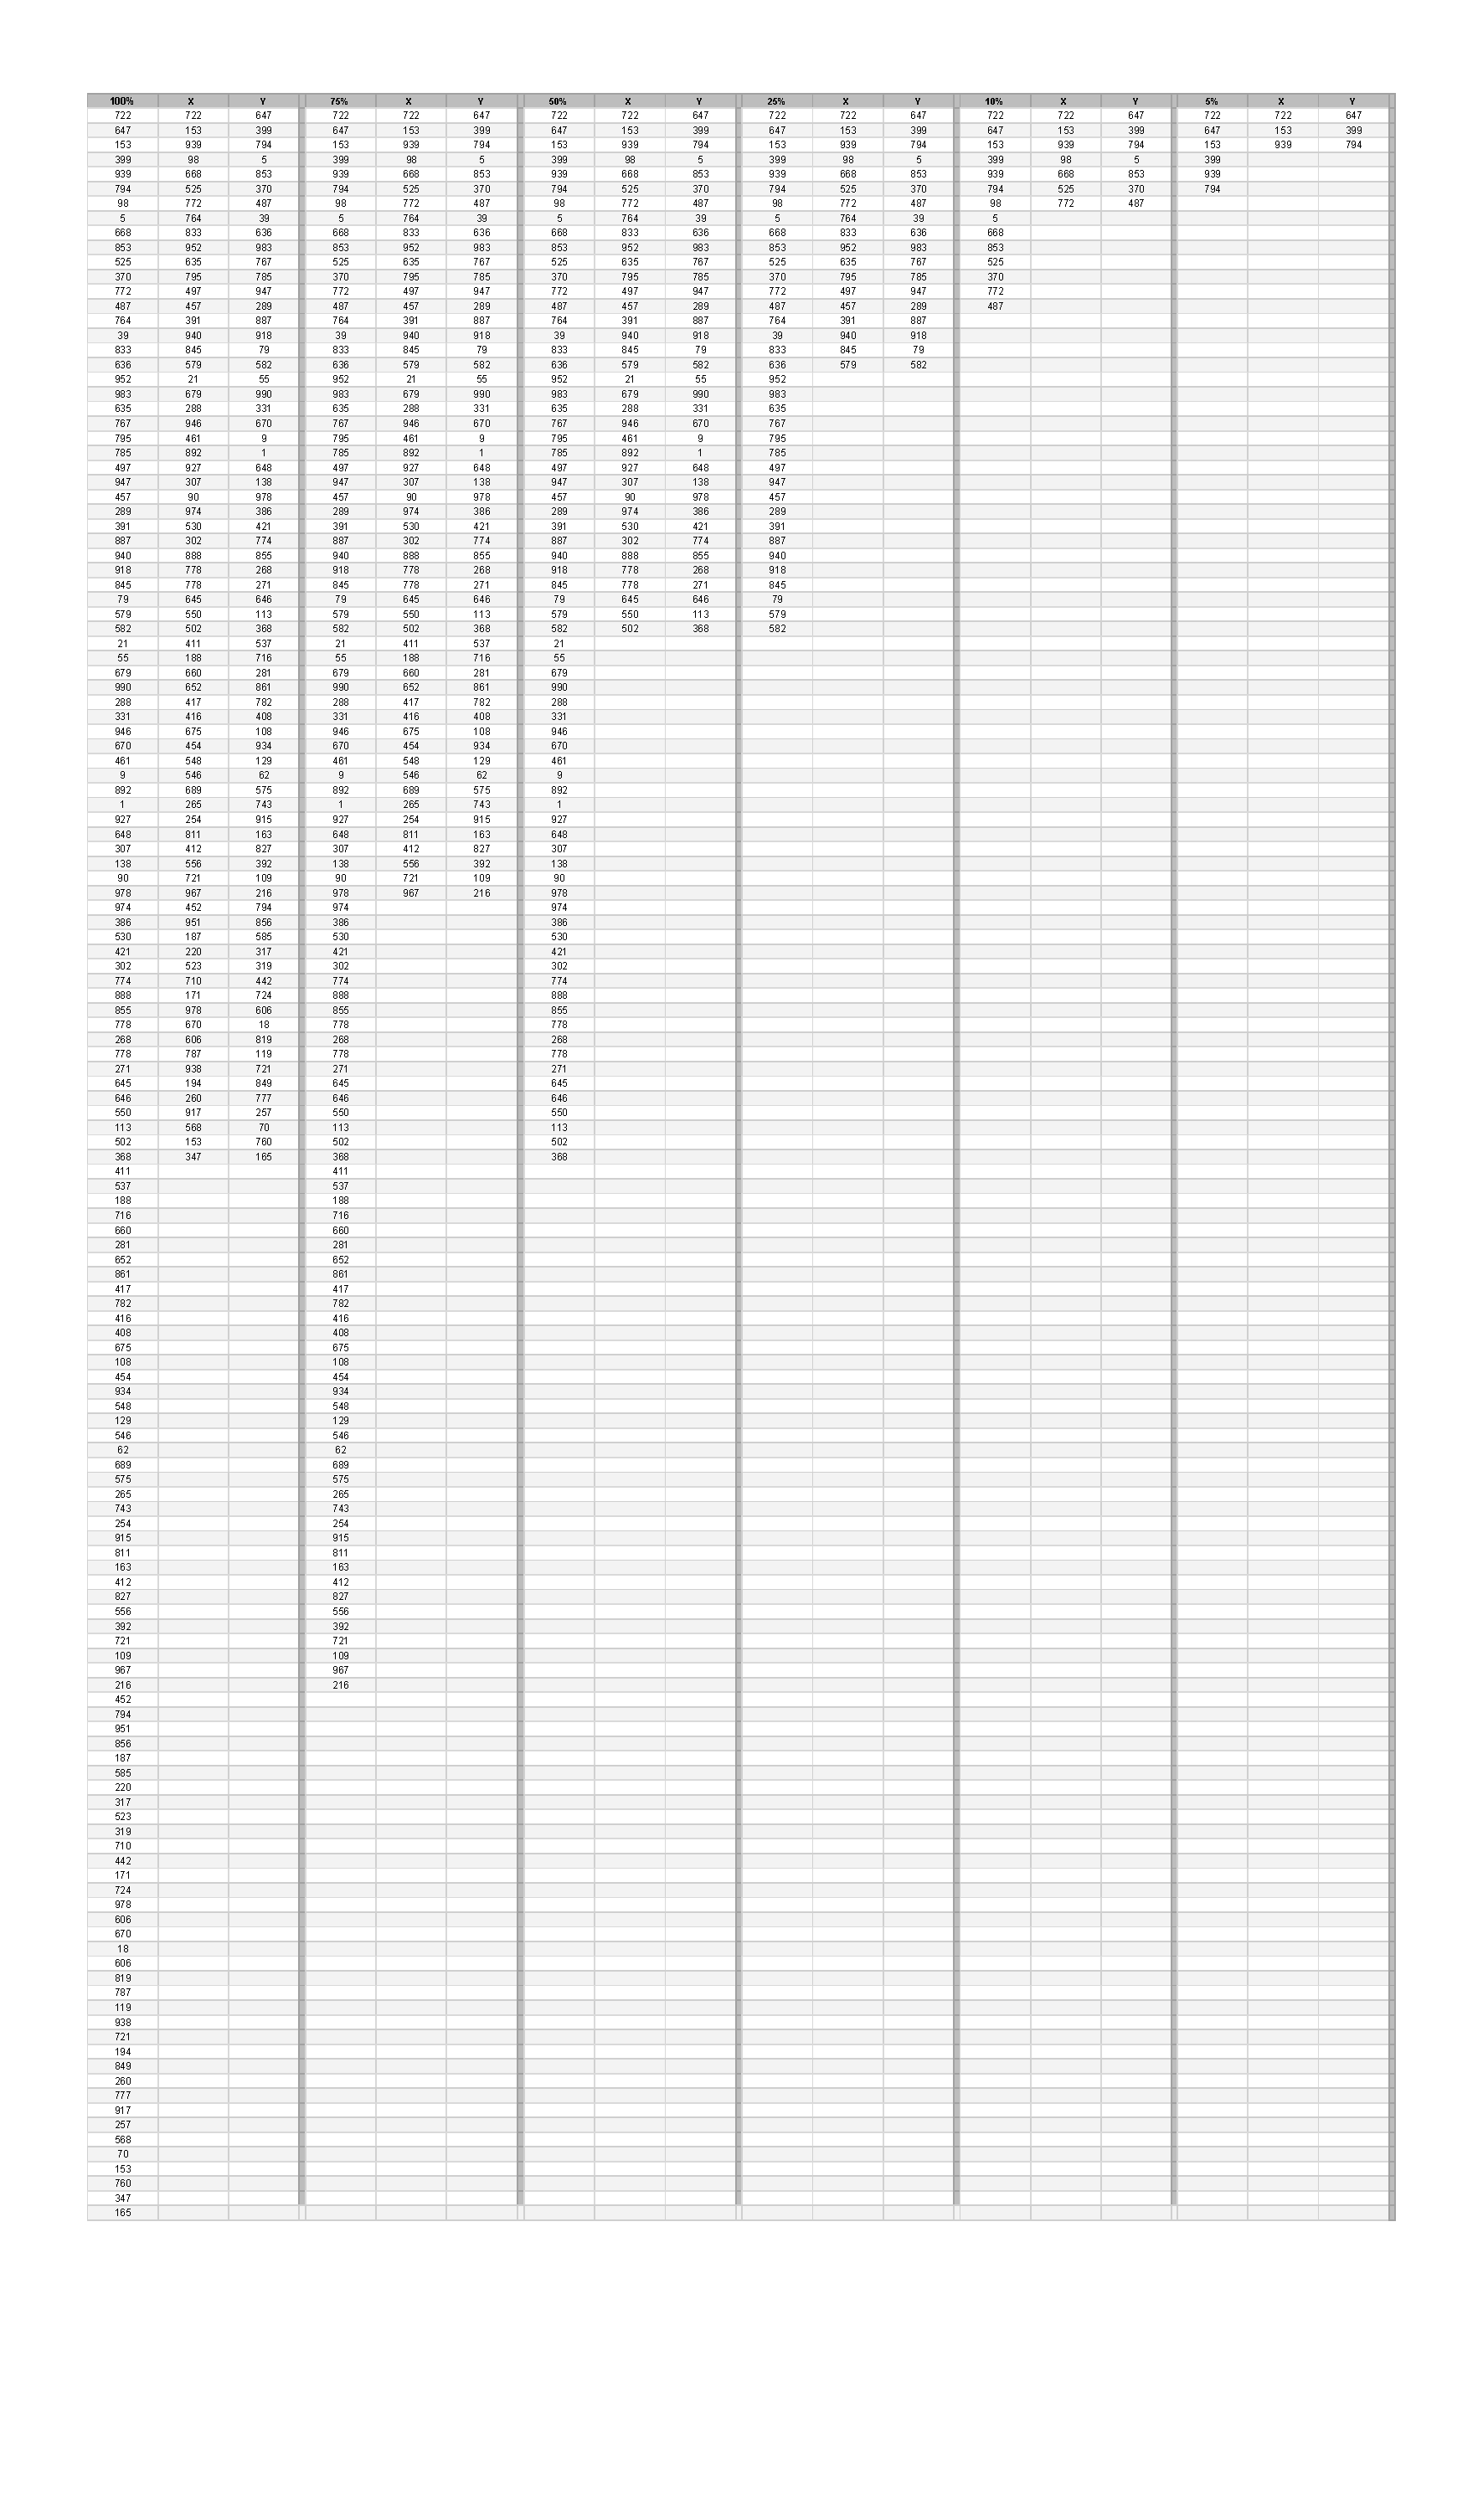
\includegraphics[width=0.74\textwidth]{tabelaRandJava.pdf}
                 \caption{Valores obtidos em um período}
                \label{fig:Desempenho}
        \end{figure}
       
Para a melhor compreensão de como é a aleatoriedade dos gráficos tanto o XorShift implementado, quanto o gerador do java, foi realizado gráficos em duas dimensões, com um par de coordenadas x e y, definido pelas seguintes periodicidades: 5\%, 10\%,25\%,50\%, 75\% e 100\%.

GRÁFICO EM XORSHIFT:

        \begin{figure}[H] 
            \centering
                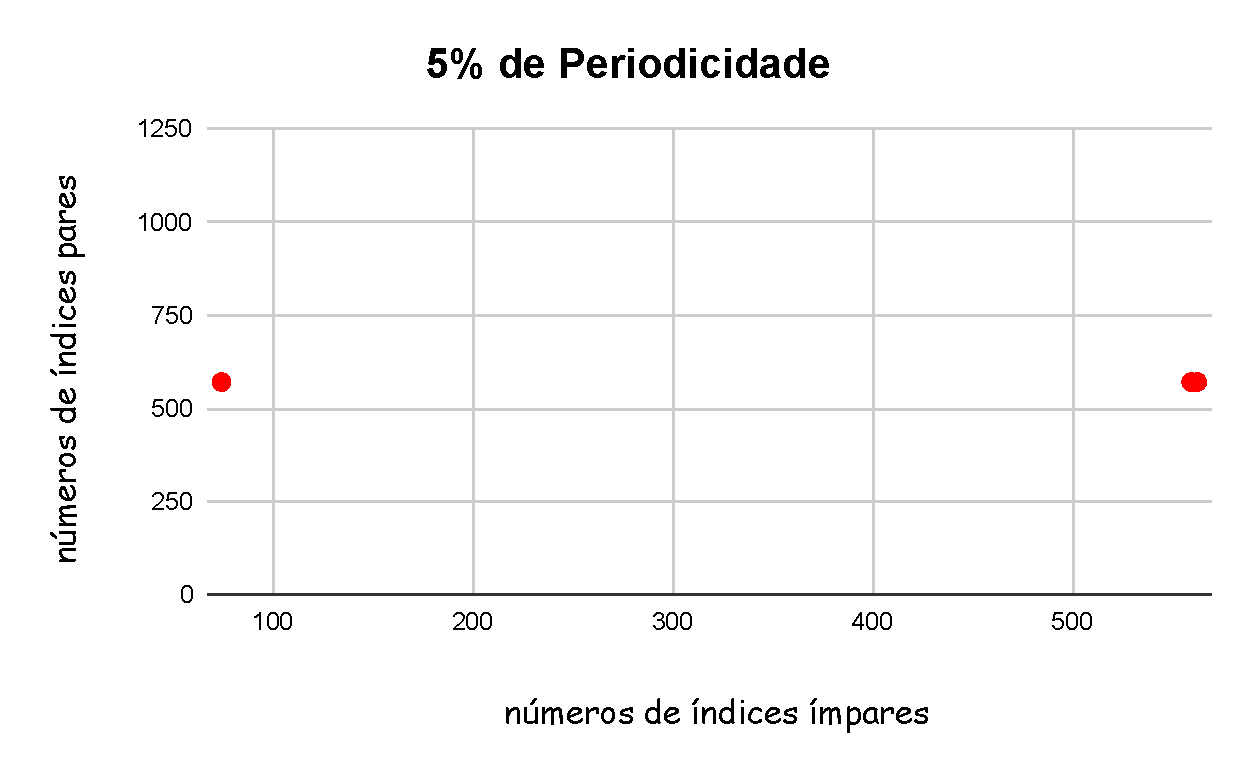
\includegraphics[width=0.496\textwidth]{5dePeriodicidade.pdf}
                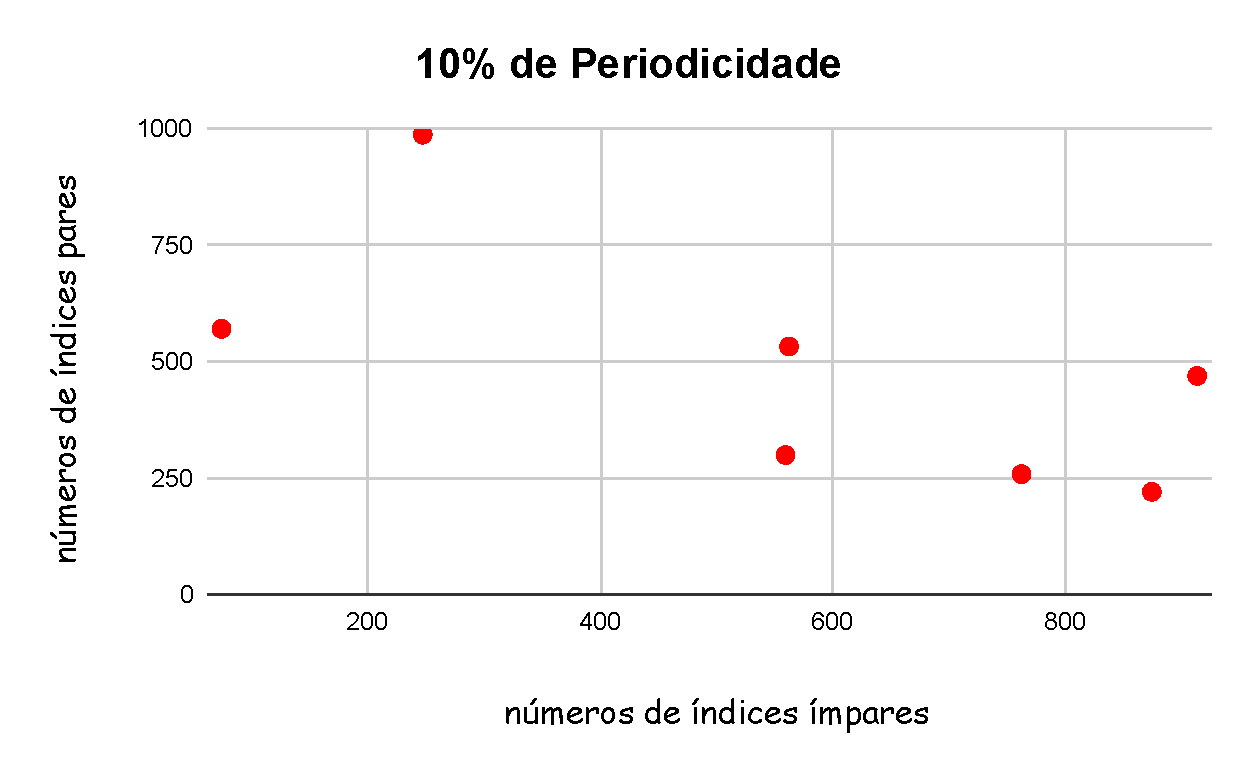
\includegraphics[width=0.496\textwidth]{10dePeriodicidade.pdf}
                \label{fig:Desempenho}
        \end{figure}
        
         \begin{figure}[H] 
            \centering
                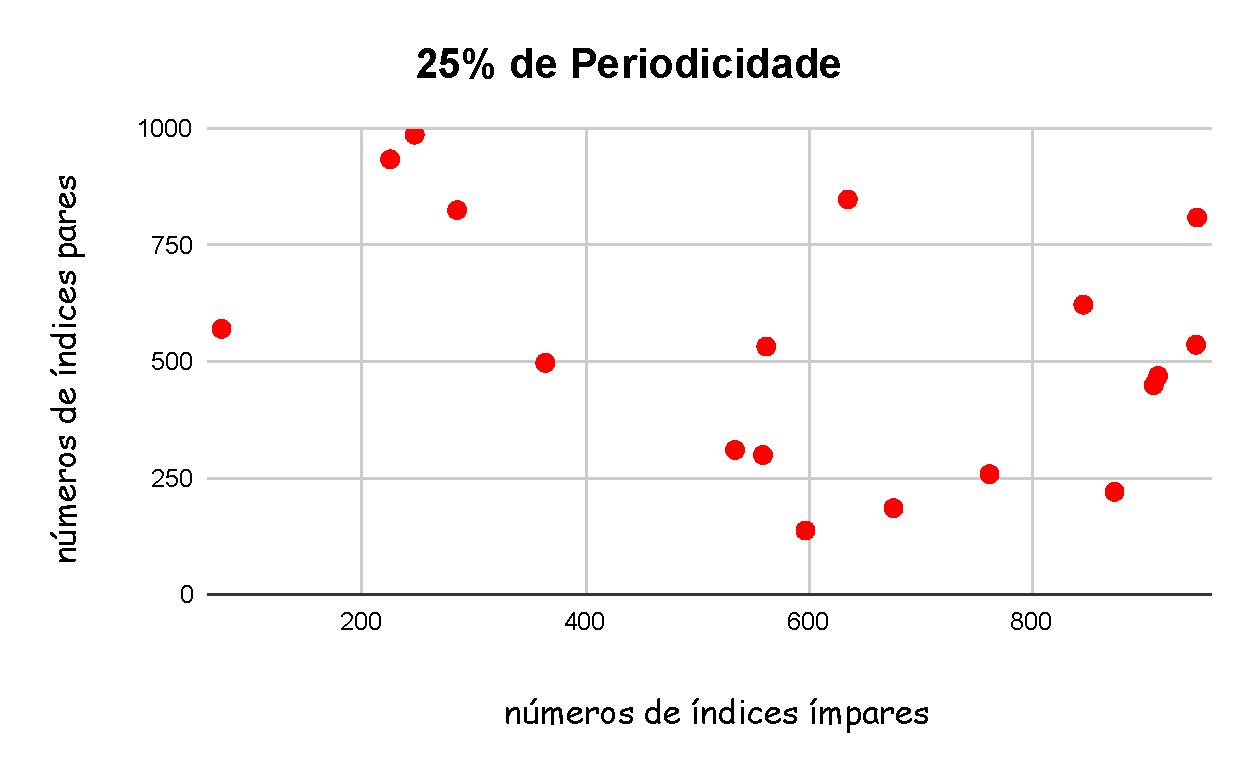
\includegraphics[width=0.496\textwidth]{25dePeriodicidade.pdf}
                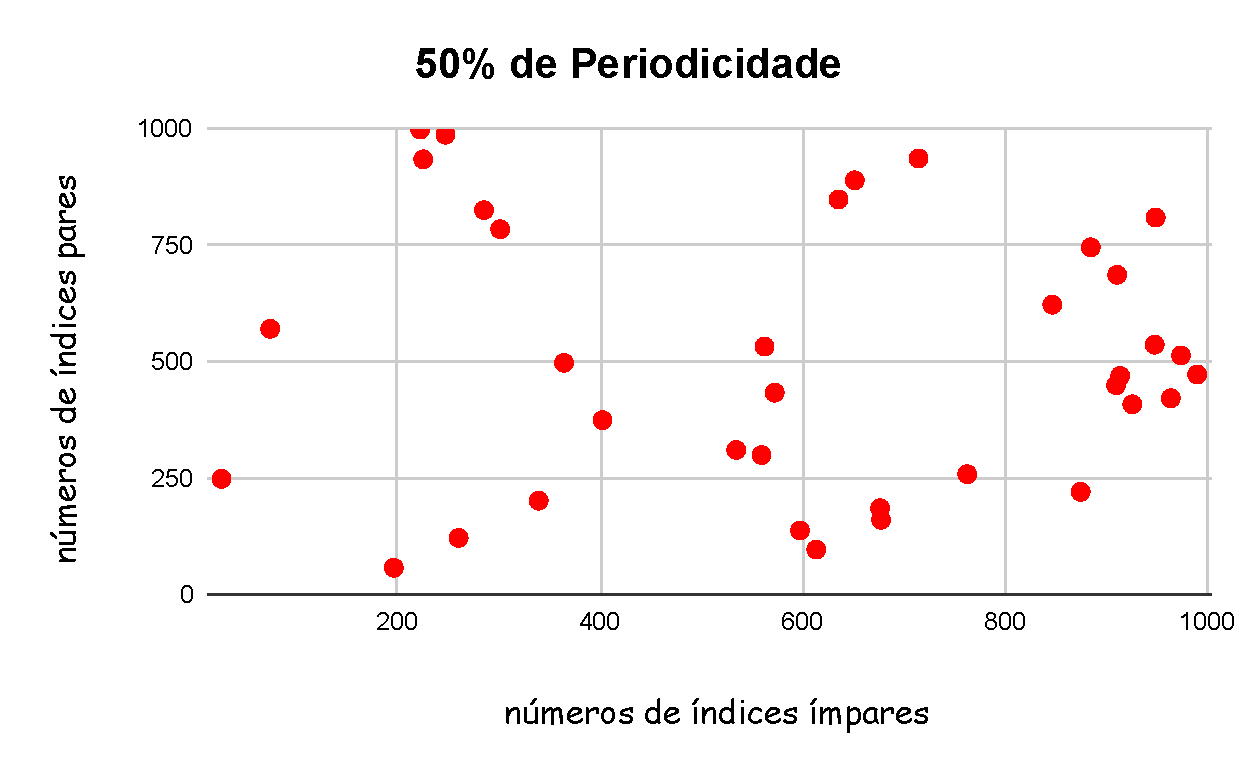
\includegraphics[width=0.496\textwidth]{50dePeriodicidade.pdf}
                     \label{fig:Desempenho}
        \end{figure}
        
         \begin{figure}[H] 
            \centering
                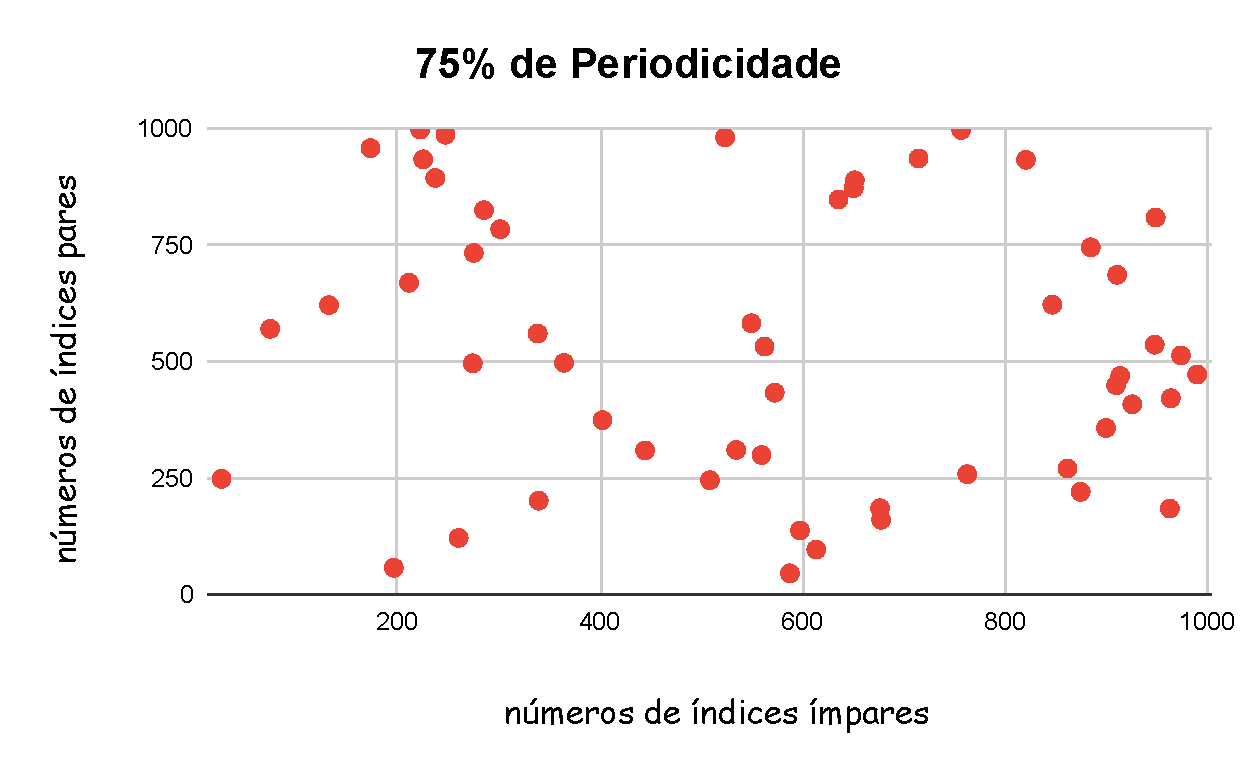
\includegraphics[width=0.496\textwidth]{75dePeriodicidade.pdf}
                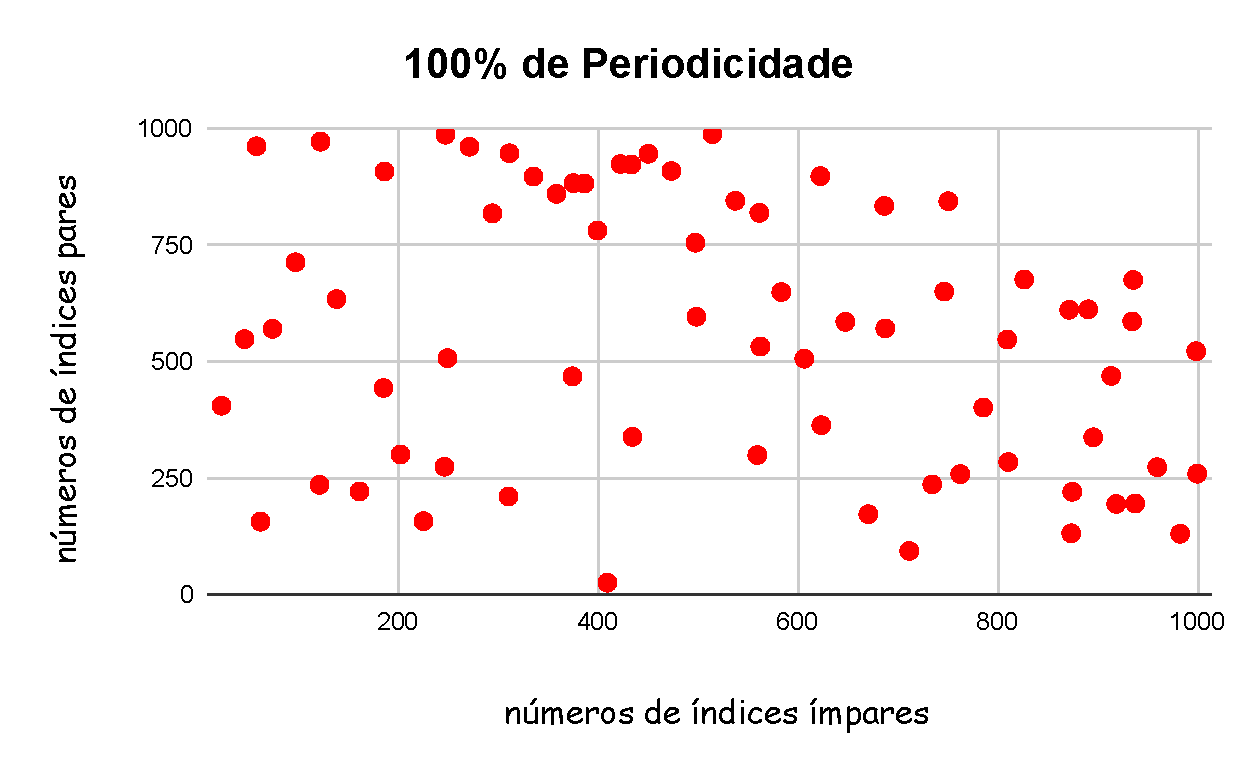
\includegraphics[width=0.496\textwidth]{100dePeriodicidade.pdf}    
                \label{fig:Desempenho}
        \end{figure}

\newpage
GRÁFICO EM JAVA:

  \begin{figure}[H] 
            \centering
                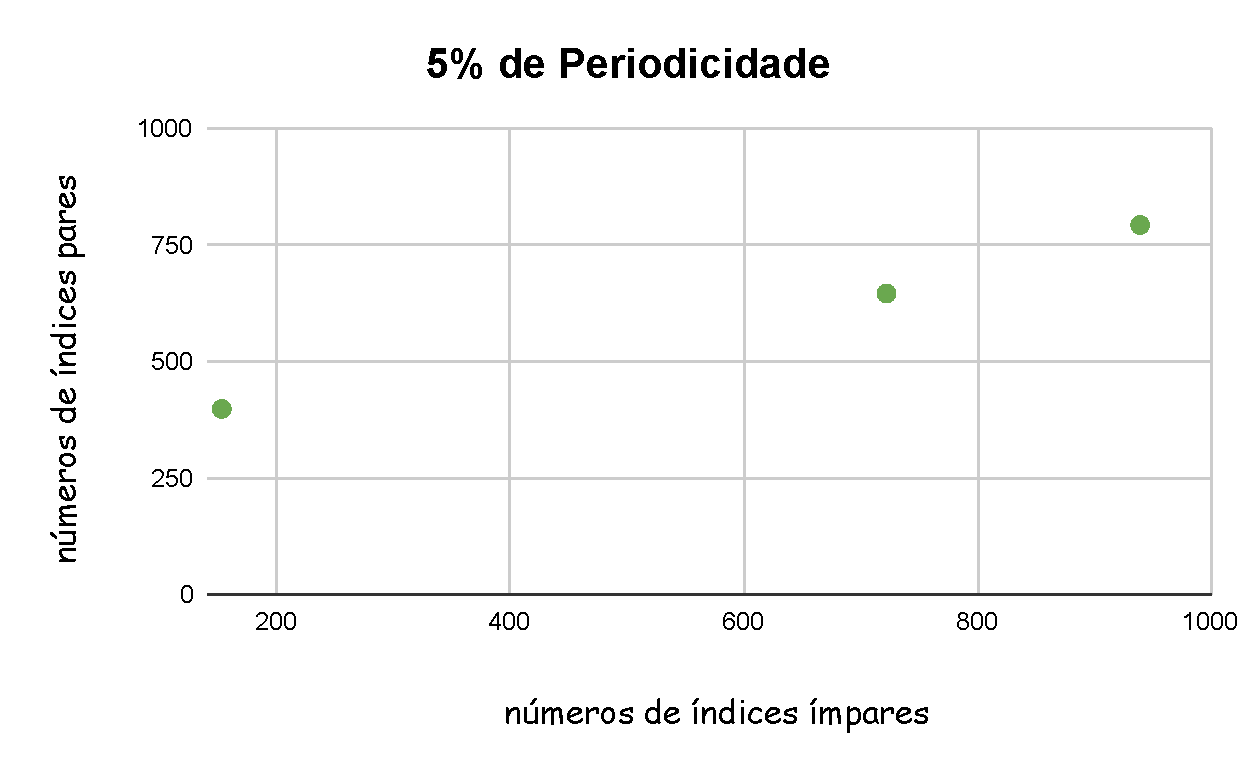
\includegraphics[width=0.496\textwidth]{5PeriodicidadeJ.pdf}
                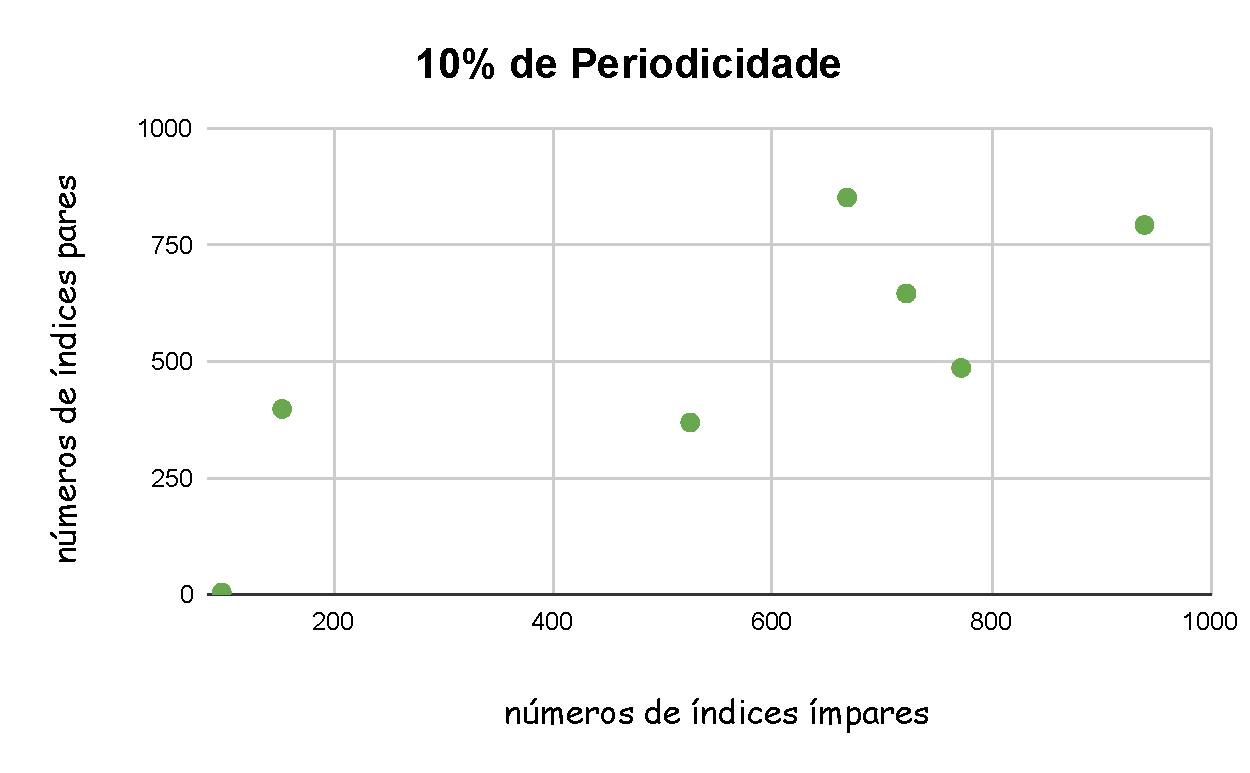
\includegraphics[width=0.496\textwidth]{10PeriodicidadeJ.pdf}
                 \label{fig:Desempenho}
        \end{figure}
          \begin{figure}[H] 
            \centering
                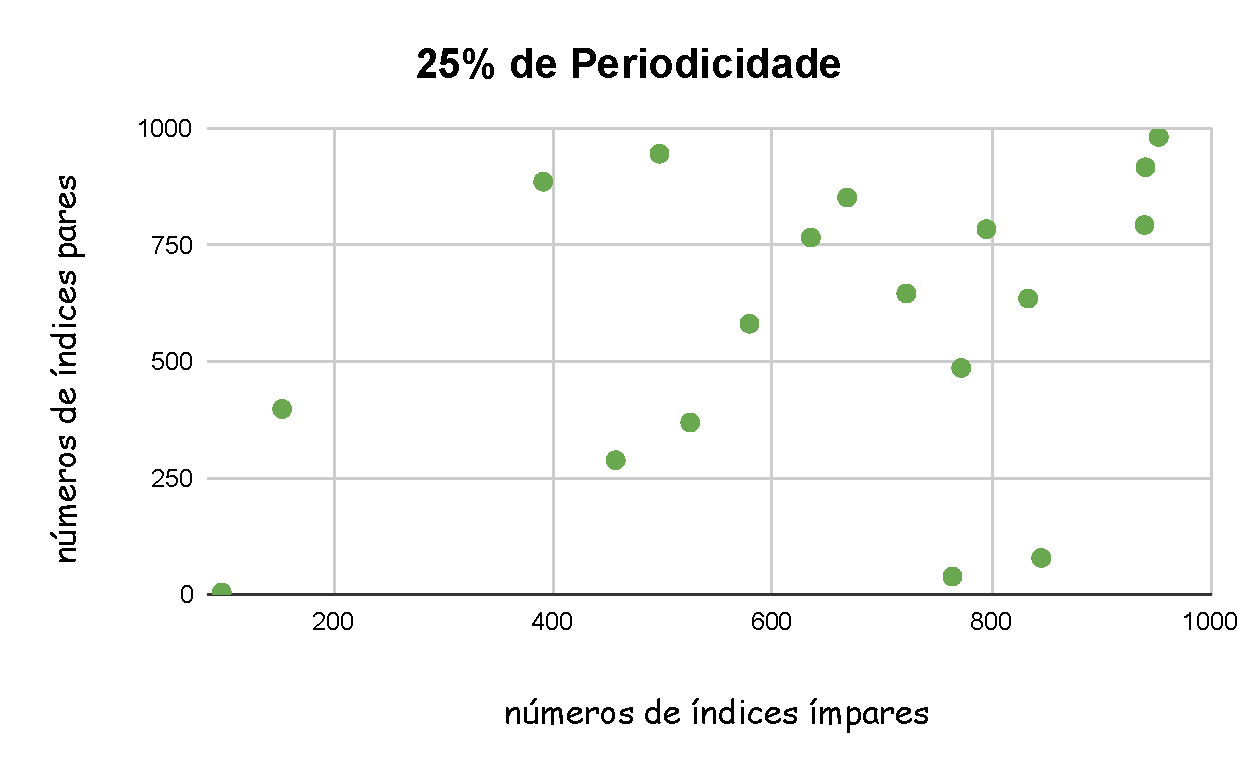
\includegraphics[width=0.496\textwidth]{25PeriodicidadeJ.pdf}
                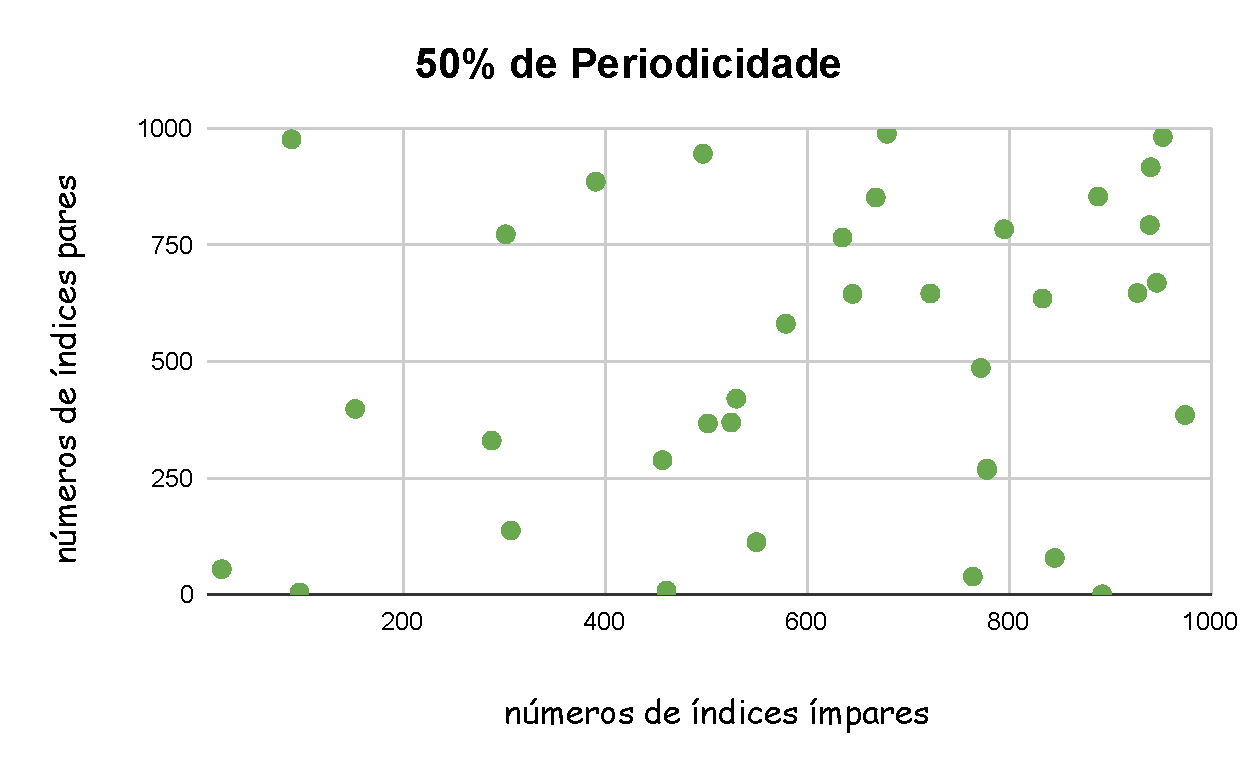
\includegraphics[width=0.496\textwidth]{50PeriodicidadeJ.pdf}
                 \label{fig:Desempenho}
        \end{figure}
          \begin{figure}[H] 
            \centering
                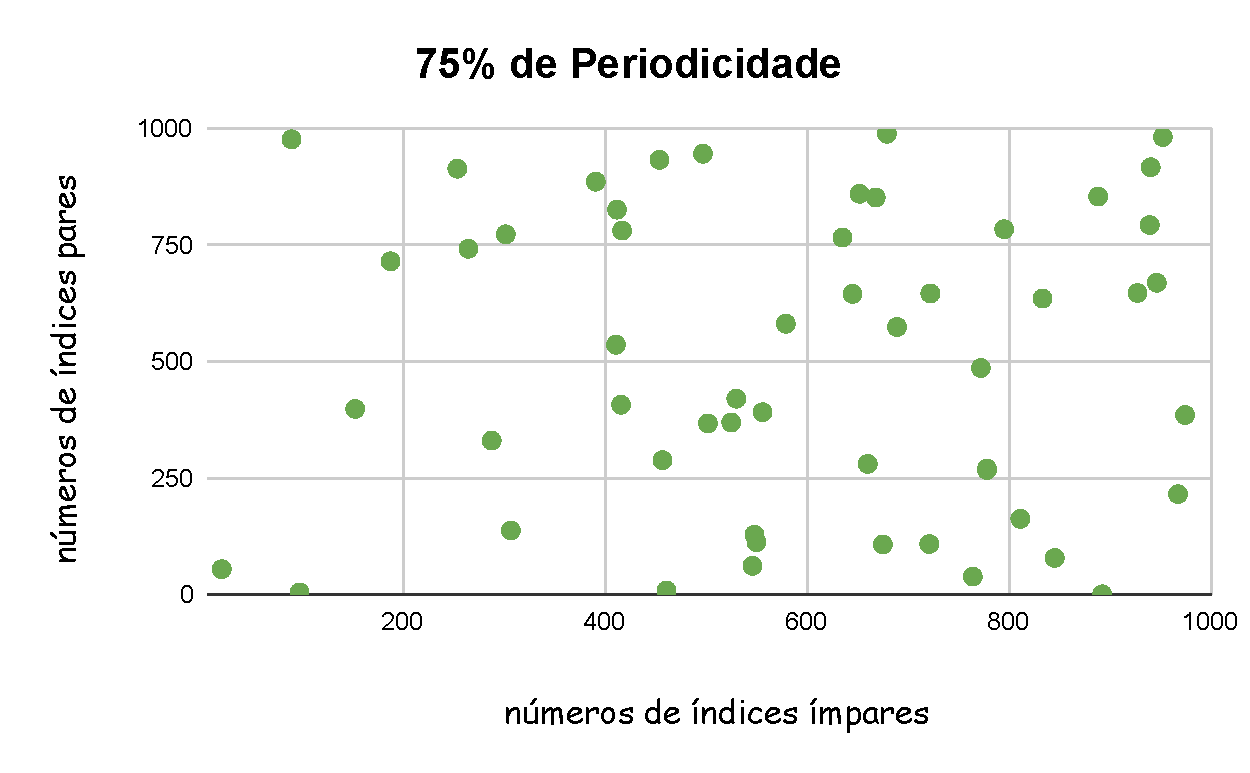
\includegraphics[width=0.496\textwidth]{75PeriodicidadeJ.pdf}
                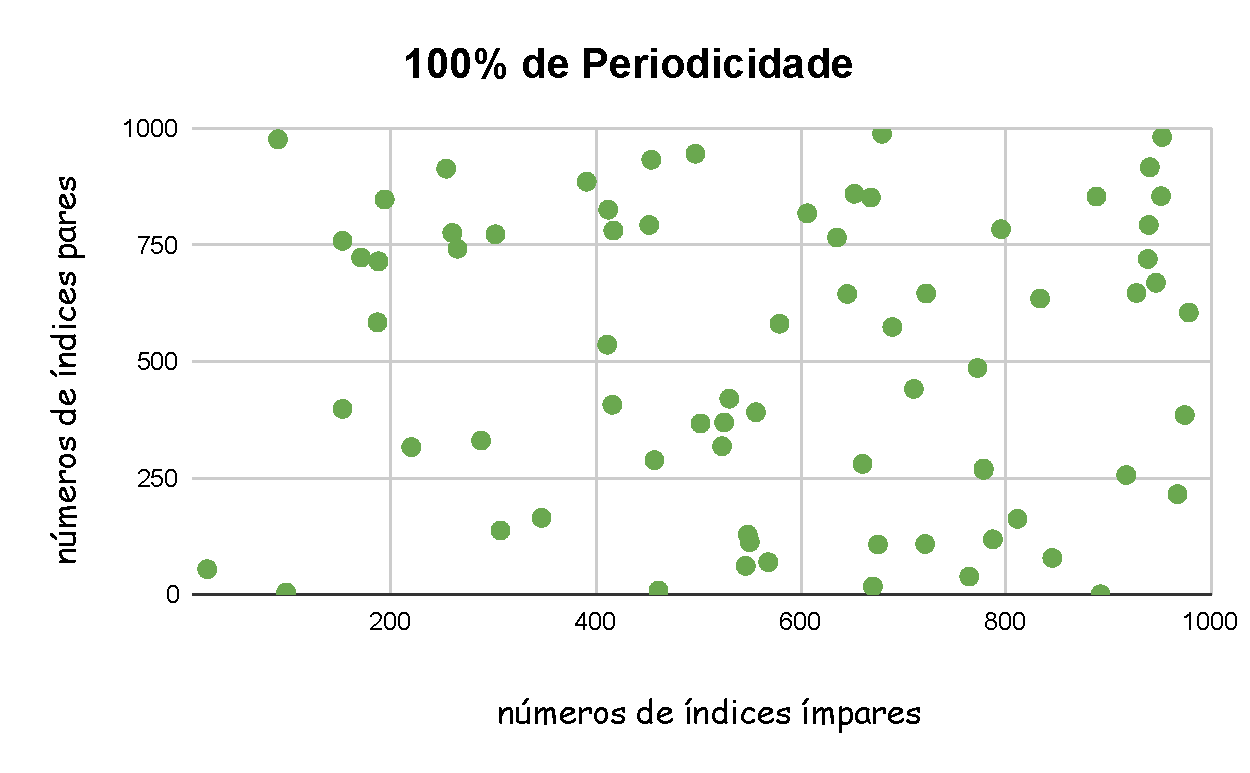
\includegraphics[width=0.496\textwidth]{100PeriodicidadeJ.pdf}    
                \label{fig:Desempenho}
        \end{figure}
        
Ao compilar os códigos, tanto o Xorshift elaborado,  quanto o Random do Java, pode-se perceber a aleatoriedade gerada por ambos, e a partir disso foi realizado os gráficos juntamente as tabelas com os devidos períodos, na execução das coordenadas,  foi empregue para os números em X os índices  ímpares da tabela - parte horizontal desta,  já para o Y os  índices pares da tabela - parte vertical desta. O gráfico do java.util.Random foi feito baseado no período do codigo xorshift, pois o período dele próprio seria grande demais.
%%%%%%%%%%%%%%%%%%%%%%%%%%%%%%%%%%%%%%%%%%%%%%%%%%%%%%%%%%%%%%%%%%%%%%%%%%%%%%%%%%%%%%%%%%%%%%%

% ---
% Finaliza a parte no bookmark do PDF, para que se inicie o bookmark na raiz
% ---
\bookmarksetup{startatroot}% 
% ---

% ---
% Conclusão
% ---
\chapter[Conclusão]{Conclusão}
\label{conclusao}
%\chapter{Conclusão} - 
Contudo, pode-se concluir que o estudo dos geradores de valores pseudo aleatórios enfatizou a noção de que valores gerados computacionalmente nunca são verdadeiramente aleatórios, pois são advindos de operações lógicas e matemáticas. Destarte, a comparação do método mais simples, Xorshift, com o código mais sofisticado de java.util.Random demonstrou que um gerador complexo, com mais operações, é melhor pois gera sequências de valores com menos padrões e coincidências.



% ----------------------------------------------------------
% ELEMENTOS PÓS-TEXTUAIS
% ----------------------------------------------------------
\postextual


% ----------------------------------------------------------
% Referências bibliográficas
% ----------------------------------------------------------
\bibliography{bibfile}

% ----------------------------------------------------------
% Glossário
% ----------------------------------------------------------
%
% Consulte o manual da classe abntex2 para orientações sobre o glossário.
%
%\glossary

% ----------------------------------------------------------
% Apêndices
% ----------------------------------------------------------

% ---
% Inicia os apêndices
% ---
%\begin{apendicesenv}

% Imprime uma página indicando o início dos apêndices
%\partapendices

% ----------------------------------------------------------
%\chapter{Quisque libero justo}
% ----------------------------------------------------------

%\lipsum[50]

% ----------------------------------------------------------
%\chapter{Nullam elementum urna vel imperdiet sodales elit ipsum pharetra ligula
%ac pretium ante justo a nulla curabitur tristique arcu eu metus}
% ----------------------------------------------------------
%\lipsum[55-57]

%\end{apendicesenv}
% ---


% ----------------------------------------------------------
% Anexos
% ----------------------------------------------------------

% ---
% Inicia os anexos
% ---
%\begin{anexosenv}

% Imprime uma página indicando o início dos anexos
%\partanexos


%\end{anexosenv}

%---------------------------------------------------------------------
% INDICE REMISSIVO
%---------------------------------------------------------------------

%\printindex

\end{document}
